% 124-17(124쪽) — $y=a\sin(bx-c)$ 의 그래프. 최댓값·최솟값 자리의 가로 점선($3$, $-3$)과 $x$절편 라벨
% $-\frac{\pi}{4}$, $\frac{\pi}{4}$(축 아래), $\frac{3}{4}\pi$(축 위), $\frac{5}{4}\pi$(축 아래)까지 원문 그대로.
% 스캔 화질이 낮아 TikZ 로 다시 그림. 원문에 없는 눈금·$a$, $b$, $c$ 의 값은 넣지 않는다.
\begin{tikzpicture}[line width=0.6pt, x=0.60cm, y=0.33cm]
  \draw[dashed, dash pattern=on 1.4pt off 1.4pt, line width=0.4pt] (-2.0,3) -- (5.95,3);
  \draw[dashed, dash pattern=on 1.4pt off 1.4pt, line width=0.4pt] (-2.0,-3) -- (5.95,-3);
  \draw[->, >=stealth, line width=0.7pt] (-2.0,0) -- (6.35,0) node[below=1pt] {$x$};
  \draw[->, >=stealth, line width=0.7pt] (0,-4.2) -- (0,4.3) node[left=1pt] {$y$};
  \draw[domain=-1.93:5.70, samples=200, smooth] plot (\x, {3*sin(114.5916*\x-90)});
  \node[anchor=south east, font=\small] at (-0.10,2.85) {$3$};
  \node[anchor=north east, font=\small] at (-0.10,-3.05) {$-3$};
  \node[anchor=north east, font=\small] at (-0.05,-0.05) {$\pt{O}$};
  \node[anchor=north east, font=\small] at (-0.72,-0.10) {$-\dfrac{\pi}{4}$};
  \node[anchor=north west, font=\small] at (0.80,-0.10) {$\dfrac{\pi}{4}$};
  \node[anchor=south west, font=\small] at (2.40,0.10) {$\dfrac{3}{4}\pi$};
  \node[anchor=north west, font=\small] at (3.95,-0.10) {$\dfrac{5}{4}\pi$};
  \node[anchor=south west, font=\small] at (2.10,3.10) {$y=a\sin (bx-c)$};
\end{tikzpicture}
